\documentclass{article}
\title{量子力学の直感 — 波であることの意味}
\author{TeX 図書館}

\begin{document}

\section{この本の目的 — 数式集ではない量子力学}

量子力学は、数式を並べただけの理論ではありません。量子力学は\textbf{「世界の見え方」そのものを変えてしまう}理論です。この本はその見え方の変化を、数式を最小限に抑えつつ、図と具体例を使ってつかませることを目的にしています。

\subsection{先に結論を述べる}

量子力学の入門書を開くと、最初に複素数や行列が並んでいます。できあがった結論は「電子は波のように振る舞う」という、たった 1 行です。しかし結論までの道は長く、その道を最初から歩くと「数式を操作している」だけで、何がどう変わったのかがつかめません。

そこで本書では順番を入れ替えます。まず「波とは何か」を、大きな波紋の図で理解します。次に「電子にも同じ性質が見つかった」という事実を先に受け入れる。そのあとで、受け入れた結論を数式 1 行に翻訳し、後ろにある理屈にさかのぼって読み解きます。

\begin{quote}
\textbf{【心構え】}\ この本を読んでも量子力学を完全に理解できるわけではありません。むしろ「わからない場所」がはっきり分かることが、この本のゴールです。わからないことを隠さないことこそ、いちばん速く理解を進める近道です。
\end{quote}

\subsection{高校物理の素養があれば足りる}

前提になるのは、高校物理の微分積分だけです。必要なのは次の 3 つだけです。
\begin{itemize}
\item 波の式 \( y = A \sin(kx - \omega t) \) を読めること
\item エネルギー \( E = \frac{1}{2} m v^2 \) を使えること
\item 指数関数 \(\mathrm{e}^{-x} \) が「急速に減る」ことを意味すること
\end{itemize}

行列も、微分方程式を解く技術も、波動方程式の解法も要りません。それらはすべて本書より後の内容であり、本書では扱いません。

\subsection{本書の約束}

本書の約束は 3 つです。
\begin{enumerate}
\item 数式は、意味を確定するために必要な最小限だけを置く。
\item 先に図と例を示し、どんな場合に電子が波に見えるかを示す。
\item 解釈(コペンハーゲン解釈、多世界解釈など)は、計算の結果ではなく視点の選択として 1 段落ずつ扱う。
\end{enumerate}

\begin{quote}
\textbf{【演習】}\ 厳密な量子力学の教科書を開いたとき、最初に現れる記号を 3 つ挙げ、それぞれ「本書は扱わない」か「扱う」かを分類せよ。
\end{quote}

\textbf{解答の指針:}\ 挙がるのは \(\psi\)、微分作用素、縦棒を並べたブラ・ケット記号などのはずです。本書が扱うのは \(\psi\)、\(|\psi(x)|^2\)、\(\Delta x \Delta p \ge \hbar / 2\)、そして重ね合わせの式 1 行までです。微分作用素とブラ・ケット記法は扱わず、第 13 節で次に何を学ぶかとして案内します。

\section{古典力学をおさらい — 「どこにいるか」が決まる世界}

\subsection{位置と速度が決まれば、その後は予測できる}

古典力学の世界では、物体の状態を 2 つの数で表せます。位置 \(x\) と速度 \(v\) です。この 2 つが決まれば、その物体の未来のすべての位置を予測できます。同じ初期状態なら、その物体は常に同じ経路をたどります。

\begin{quote}
\textbf{【定義:古典力学】}\ 物体の状態を位置 \(x\) と速度 \(v\) だけで表し、それらに従う法則から将来の運動が一意に決まるという考え方。
\end{quote}

\subsection{ニュートンの運動方程式}

物体の運動を変えるのは力です。質量 \(m\) の物体に力 \(F\) がはたらくと、加速度は
\[ a = \frac{F}{m} \]
となります。位置と速度の時間変化は
\[ \frac{dx}{dt} = v, \qquad m \frac{dv}{dt} = F(x, t) \]
のように書けます。右辺に「今いる場所」と「時刻」しか現れないのが要点です。力学は、その瞬間の合力だけを見て、現在と未来を決めるという形になっています。

\begin{quote}
\textbf{【例:月と地球以外の力】}\ 地球を回る人工衛星の軌道を考えます。ニュートン力学で計算すると、月や太陽からの重力が無視できないため、実際の軌道とはわずかにずれます。このずれは一般相対論の補正で説明できます。ニュートン力学が近似にすぎないことの例であり、位置と速度だけがあれば十分だという仮定の輪郭が見えてきます。
\end{quote}

\subsection{古典力学が成り立つ 2 つの前提}

古典力学の世界は、ちょうど 2 つの仮定で立っています。
\begin{itemize}
\item \textbf{決定的}: 位置と速度が決まれば、その将来は一意に決まる。
\item \textbf{局所性}: 物体に影響するのは今ここにあるものだけで、遠くの過去は直接は見えない。
\end{itemize}

この 2 つは、粒子が「ちょうどそこにある」ことを前提にしています。粒子が持っているのは、場所と速さ、そしてその場での相互作用だけです。

\begin{quote}
\textbf{【注意】}\ 気体の分子の運動を観測すると、分子 1 個ずつの位置は予想できないのに、多数を重ねると整った分布が現れます。決定的という前提が分子のスケールでは見えないということは、観測者の選び方による問題だという量子力学の言い換えを、ささやかに予感させるだけのものです。
\end{quote}

\begin{quote}
\textbf{【演習】}\ 古典力学の 2 つの仮定(決定的・局所性)を、卓球の例を使って 1 つずつ説明せよ。
\end{quote}

\textbf{解答の指針:}\ 決定的とは、ボールの位置と速度が分かれば以後は必ず同じ軌道をたどる、という意味です。局所性とは、その場の情報だけで力学を計算でき、遠くの過去の情報は直接では効かない、という意味です。この 2 つが崩れることが、以降の量子力学のすべてです。

\section{光は波か、粒子の問い — ヤングのスリット実験}

\subsection{ヤングのスリット実験}

長い間、光の正体は決まっていました。17 世紀のニュートンは、光は微小な粒子の集まりであると考えました。しかし 19 世紀末、ヤングとフレネルが精密な実験によって干渉を説明し、光が波であることを示します。

この実験の装置は単純です。明るい一点光源の前に、スリットを 2 つ開けた板を垂直に置き、光を当てる。スリットを通った光は、2 つのスリットを点光源として広がって進みます。スクリーンには、明線と暗線が交互に現れます。この縞を干渉縞と呼びます。

\begin{figure}[h]
\centering
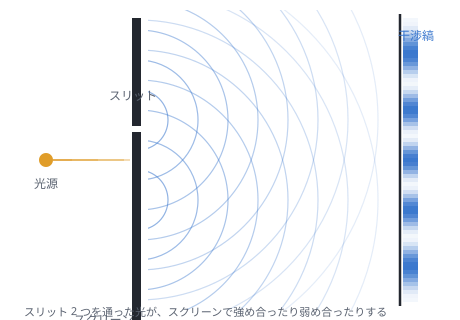
\includegraphics[width=0.78\textwidth]{figures/slit.svg}
\caption{ヤングのスリット実験。スリット 2 つを通った光がスクリーン上で強め合ったり弱め合ったりして、干渉縞をつくる。}
\end{figure}

\subsection{干渉縞の正体}

明線と暗線が等間隔に並んでいるのが、この実験の一番の特徴です。山と山が常に同じだけずれたところで重なるため、縞の間隔が波の波長に比例します。スクリーン上の縞の間隔を測れば、光の波長が分かる。波長を測れるなら、そこには波がある。

プールに石を 1 つ投げても同じことが起こります。石を中心とする同心円の波紋は、2 つの場所から来た波と重なり、明暗の模様をつくります。干渉縞とは、その縞模様そのものです。

\subsection{粒子説では説明できない}

では、光が「とても小さな弾丸の連なり」だったら、スクリーンに何が見えるか考えてみます。弾丸なら、スリットを通ったものだけが光ります。光る点は 2 本の帯になり、縞にはなりません。

\begin{quote}
\textbf{【演習】}\ スリットを 2 つ通った光がスクリーン上で干渉縞をつくることは、光を粒子の弾丸とみなしたすべてでは説明できません。弾丸説で予想されるスクリーン上の模様を書き、実際の縞とどこが違うか述べよ。
\end{quote}

\textbf{解答の指針:}\ 弾丸説なら明点はスリットの真下に来る 2 本の帯になります。その幅はスリットの幅とほぼ同じです。現実には明点が数十本も等間隔に並んでいます。1 つの粒子が 1 か所にしか当たらない以上、複数の波が重なって干渉する仕組みを導入しない限り、この 1 本ずつの縞は説明できません。

\section{電子も波だった — ド・ブロイの関係}

\subsection{光は波であると同時に粒子である}

20 世紀に入り、光が波であるだけでは足りないことが分かりました。光電効果という現象をアインシュタインが 1905 年に説明したためです。光が粒子であるとして、光子のエネルギー \( E = h \nu \) で金属から電子が飛び出すと説明できたのです。つまり光は、波であると同時に粒子でもあります。

\begin{quote}
\textbf{【補足】}\ ここでいう粒子とは、光のエネルギーと運動量がひとまとまりで伝わる、という意味です。見えている小球であるという意味ではありません。波か粒子かではなく、どちらの側面も実在する、というのがこの時期の結論です。
\end{quote}

\subsection{ド・ブロイの関係}

1924 年、ド・ブロイは逆に提案しました。粒子と波は同じものではないかと。粒子が運動量 \(p\) をもつなら、それには波長
\[ \lambda = \frac{h}{p} \]
が対応します。ちょうど、光の粒子である光子が波長 \(h / p\) をもつのと同じ式です。定数 \(h\) はプランク定数で、
\[ h = 6.626 \times 10^{-34} \ \mathrm{J \cdot s} \]
という、極めて小さい数です。

\begin{quote}
\textbf{【定義:ド・ブロイ波長】}\ 運動量 \(p\) をもつ粒子に対応する波長をド・ブロイ波長といい、\( \lambda = h / p \) と書く。運動量が大きいほど波長は短くなる。
\end{quote}

\subsection{電子の波長はどれくらいか}

では、どれほどの速さで飛ばすと、どれほどの波長になるのか。100 V の電圧で加速した電子を例に取りましょう。運動エネルギーと運動量は
\[ p = \sqrt{2 m E} \]
で結びつきます。電子の質量は \(9.11 \times 10^{-31} \ \mathrm{kg} \)、100 eV は \(1.60 \times 10^{-17} \ \mathrm{J} \) なので、\(p \approx 5.4 \times 10^{-24} \ \mathrm{kg \cdot m/s} \)、波長は
\[ \lambda = \frac{h}{p} \approx 1.2 \times 10^{-10} \ \mathrm{m} \]
となります。これは原子の大きさそのものです。原子の大きさは 0.1 nm 程度ですから、ちょうど同じスケールです。

\begin{quote}
\textbf{【例:電子の回折】}\ この干渉の実験は 1961 年ごろ、数十 kV で加速した電子を微細な結晶に当てました。結晶は原子が規則正しく並んでいるため、原子間隔に等しい回折格子として働きます。電子の波長が原子間隔と一致するときだけ、明瞭な模様が出ます。この実験は、電子にも波長があることを直接示す証拠です。
\end{quote}

\subsection{日常の物体は波にならないのか}

目に見える物体ではどうでしょうか。\(h\) は \(10^{-34}\) という小さい数なので、\(\lambda = h / p\) はもっと小さくなります。鋼製の針の質量を \(1 \ \mathrm{mg} = 10^{-6} \ \mathrm{kg} \)、速さを \(1 \ \mathrm{m/s} \) とすると、
\[ \lambda = \frac{6.626 \times 10^{-34}}{10^{-6}} = 6.6 \times 10^{-28} \ \mathrm{m} \]
です。これは原子の大きさの約 \(10^{-18}\) 倍になります。

\begin{quote}
\textbf{【注意】}\ 自分には波長がない、というわけではありません。日常の物体にもド・ブロイ波長は存在します。ただしその波長は観測装置の限界より何桁も小さく、原理的に検出できません。電子が波だから見つからないのではなく、同じ式が波として見える値と見えない値との境目を決めているのが、正確な説明です。
\end{quote}

\begin{quote}
\textbf{【演習】}\ 速さ \(1.0 \times 10^{6} \ \mathrm{m/s} \) で飛ぶ電子のド・ブロイ波長を見積もりよ。電子の質量を \(9.11 \times 10^{-31} \ \mathrm{kg} \) とする。加えて、同じ電子の速さを 10 倍にすると波長は何倍になるか答えよ。
\end{quote}

\textbf{解答の指針:}\ 運動量は \(p = mv = 9.11 \times 10^{-25} \ \mathrm{kg \cdot m/s} \) なので、\(\lambda = 6.626 \times 10^{-34} / 9.11 \times 10^{-25} \approx 7.3 \times 10^{-10} \ \mathrm{m}\)、約 0.73 nm です。これは原子の 7 倍ほどになります。\( \lambda = h / p \) で \(p = mv\) なので、波長は速さに反比例します。よって速さが 10 倍なら、波長は 10 分の 1 倍になります。

\section{二重スリット実験 — 電子を 1 個ずつ発射する}

\subsection{1 個ずつ発射する}

ここが本書の中心となる実験です。前の節の光ではなく、電子を使います。電子源を改造し、1 秒に 10 個ほどの極めて遅い速さで、電子を 1 個ずつ放出する装置を作ります。そして 2 つのスリットと、その先のスクリーンを用意します。電子 1 個がスクリーンに当たって点が 1 つ光ったことを記録し、それを繰り返します。

\subsection{何十個も重なると現れるもの}

最初は 1 個の点。10 個では 10 個の点。100 個でもまだ模様は見えません。電子を 1 万個ほど重ねると、スクリーンにははっきりと干渉縞が現れます。電子 1 個 1 個は、スクリーン上の 1 点にしか当たりません。それなのに、多数の点の分布には明暗の縞が刻まれています。

\begin{figure}[h]
\centering
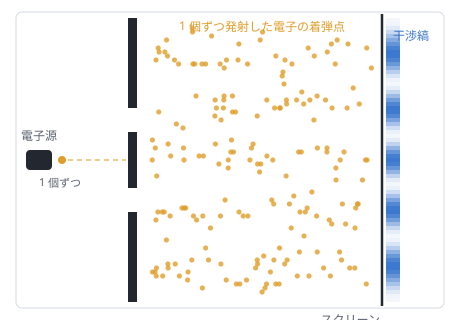
\includegraphics[width=0.72\textwidth]{figures/doubleslit.svg}
\caption{電子を 1 個ずつ発射し、多数回の着弾点を重ねる。スクリーンには干渉縞が現れる。}
\end{figure}

\subsection{1 個ずつと多数の緊張}

ここに残っている矛盾です。電子 1 個は、スクリーン上の 1 点にしか当たりません。1 個の電子の記録には、干渉縞のかけらがありません。しかし多数の記録を重ねると、その 1 個の電子の記録が明暗の縞をつくりました。各電子は、自分 1 個では縞を作れなかったのです。

\begin{quote}
\textbf{【例:砂浜の脚印】}\ 砂浜に 1 つずつ脚印を残して行くと、砂の凹凸は点々です。1 人だけが歩いても、砂に縞は残りません。何人かが同じ場所を続けて歩いて、ようやく砂の凹凸に模様が見えてきます。干渉縞は、電子 1 個 1 個の記録が同じ場所に集中した結果です。
\end{quote}

\begin{quote}
\textbf{【注意:これは矛盾ではない】}\ 1 個ずつ発射したのに干渉縞が現れることは矛盾ではありません。矛盾が起きたのは、電子 1 個がどれか 1 つのスリットを通ったものと思う前提が誤っていたためです。この前提を捨てれば、2 つのスリットを通る可能性が重なっている、と説明できます。これが次の節の主題です。
\end{quote}

\begin{quote}
\textbf{【演習】}\ 電子を 1 個ずつ発射する二重スリット実験で、電子を 1 個だけ発射した場合と 100 個発射した場合のスクリーン上の模様を、それぞれ記述せよ。加えて、干渉縞の実験から電子の経路が分かるかどうかを述べよ。
\end{quote}

\textbf{解答の指針:}\ 1 個なら点 1 つです。100 個ならまだ縞は目立ちませんが、確率的な偏りはわずかに現れます。経路は分かりません。どれがどちらのスリットを通ったかを後から調べる装置を仕掛けると、干渉縞は消えて単に 2 本の帯になります。記録そのものからは経路の情報を取り出せない、というのが要点です。

\section{観測の問題 — 「観測」とは何か}

\subsection{観測とは何か}

ここで混乱しやすい言葉を分解します。観測とは、目で見ることだけではありません。検出器が電子を捉えたことも観測です。現実には、電子がどこで吸収され、どんな情報が受け取ったかが観測の本体です。目やカメラ、測定器は、その情報を受け取る便利な道具にすぎない。

\begin{quote}
\textbf{【定義:観測の便宜的な意味】}\ 粒子の状態が、ある場所と時間に関する明確な情報として取り出されたとき、その取り出しを観測と呼びます。情報を取り出す装置を情報源と呼びます。
\end{quote}

\subsection{通過を確定する装置}

二重スリットの各スリットの直後に、電子がどちらを通ったかを示す装置を付けます。スリットの近傍に検出器を置き、電子が触れたほうを記録します。すると何が起きるか。スクリーンには干渉縞が現れず、単に 2 本の帯が現れます。どちらを通ったかが確定すると、その 2 つの道筋は干渉できなくなるのです。同じ装置なのに、付けるだけで結果が完全に変わります。

\begin{quote}
\textbf{【補足】}\ 観測者が人間である必要はありません。装置でも、他の粒子でも、記録媒体でも構いません。重要なのは、結果が 1 つに定まる情報として取り出されたかどうかです。
\end{quote}

\subsection{ゼノ効果 — 観測の回数を増やす}

観測を細かい時間間隔で繰り返すと、驚くことが起こります。観測の回数を増やすのではなく、観測の時刻をきわめて短くすると、崩壊の確率が下がります。不安定な状態にある粒子を短い間隔で観測し続けると、崩壊させずに保てるのです。見つけるのが早ければ見つからない、というのがゼノ効果です。

\begin{quote}
\textbf{【例:励起状態の原子】}\ 励起された原子は、平均的な寿命の時間を経て自ら崩壊します。100 回観測すれば、そのうち 1 回で崩壊します。しかし観測間隔を 1 ピコ秒程度まで短くすると、事実上崩壊させずに原子を保持できます。可視光の波長スケールです。
\end{quote}

\subsection{観測は破壊ではなく関係}

観測すると波が崩れるという言い方は、誤解を招きます。波が壊れるのではなく、装置と粒子が関係した時点で、干渉できる情報が失われるというのが正確な説明です。装置は粒子の重みの情報を受け取って、1 つの結果にする、というしくみなのです。この関係は一方的ではありません。装置も粒子に変えられます。衍射測定では、装置も量子状態をもっています。

\begin{quote}
\textbf{【演習】}\ 二重スリット実験で、一方のスリットの直後だけに検出器を付けた。このときスクリーンにできる模様を書き、検出器が無い場合とある場合の違いを、それぞれ 1 文で説明せよ。
\end{quote}

\textbf{解答の指針:}\ 検出器が無い場合は干渉縞になり、明線が多数現れます。ある場合は 2 本の帯になり、明点は 2 箇所に偏ります。どちらのスリットを通ったかが確定する情報が残ると、2 つの道筋を重ね合わせる干渉計算ができなくなるためです。ここで失われるのは波そのものではなく、干渉を計算するための前提です。


\section{波関数と確率振幅 — 「可能性の重み」をもつ波}

\subsection{波関数とは}

ここからは少し数式に入ります。使う式は 1 本だけです。

\begin{quote}
\textbf{【定義:波関数】}\ 量子的な粒子の状態を表す複素数の関数を波関数といいます。位置 \(x\) に電子がいるという可能性を、波関数 \(\psi(x)\) が表します。\(\psi(x)\) は電子そのもの」ではなく、\(x\) にいるという可能性を表します。
\end{quote}

\subsection{絶対値の 2 乗が確率密度}

中心となるのは、次の 1 文です。

\begin{quote}
\textbf{【定義:Born ルール(概略)】}\ 位置 \(x\) の近く、つまり幅 \(\mathrm{d}x\) の区間に電子が見つかる確率は、\(|\psi(x)|^2\) に比例します。
\end{quote}

\begin{quote}
\textbf{【補足】}\ 波関数 \(\psi\) そのものは確率ではありません。確率になるのは、その絶対値を 2 乗した \(|\psi|^2\) です。この区別が、二重スリットを理解するための最大のポイントです。
\end{quote}

\subsection{振幅と確率の違い}

なぜ 2 乗が必要になりますのか。波関数は複素数だからです。複素数には、大きさだけでなく、向きに由来する位相も付きます。山と山が重なるか、山と谷が重なるかは、この位相で決まります。位相がなければ、干渉という現象は原理的に起こりません。位相を区別しない単純な足し算では、この干渉は起こりません。

\begin{quote}
\textbf{【要点】}\ 波関数は確率の重みではなく、複素数としての位相を持ちます。位相があるため、2 つの可能性を重ねたときに強め合う場所と打ち消し合う場所が区別されます。
\end{quote}

\subsection{二重スリットを読み直す}

これで第 5 節の実験が説明できます。電子 1 個は、左のスリットを通る可能性と右のスリットを通る可能性の 2 つをもっています。この 2 つの可能性は、それぞれ 1 つの波関数として書けます。

この 2 つの可能性が同じ場所で重なると、位相が合う場所では強くなり、位相がずれる場所では打ち消されます。その強さの分布が、スクリーン上の干渉縞そのものです。電子 1 個の着弾点が、重なる場所ほど当たりやすい分布に従う。多数の点がこの分布的平均を取ると、干渉縞が現れます。

\begin{quote}
\textbf{【演習】}\ \(\psi(x) = 0.3\,\mathrm{e}^{\mathrm{i}0}\mathrm{e}^{-x/2}\) を考え、\(\mathrm{i} = \sqrt{-1}\) として、\(|\psi(x)|^2\) を求めよ。加えて、位相の因子 \(\mathrm{e}^{\mathrm{i}0}\) を落としたときの確率密度との違いを述べよ。
\end{quote}

\textbf{解答の指針:}\ 絶対値を 2 乗するので位相の因子は消え、\(|\psi(x)|^2 = 0.09\,\mathrm{e}^{-x}\) となります。\(x = 0\) で最大になり、右に向かって指数的に減る分布です。位相の因子 \(\mathrm{e}^{\mathrm{i}0} = 1\) を落としても、確率密度は変わりません。ただし位相は、2 つの波を重ねたときの干渉には効きます。\(|\psi|^2\) だけを見ると位相は隠れてしまう、というのが要点です。

\section{重ね合わせと干渉 — 古典力学にない項}

\subsection{重ね合わせという考え方}

2 つの可能性を重ねるとき、確率を足し合わせるのではありません。波関数を足し合わせます。

\begin{quote}
\textbf{【定義:重ね合わせ(線形性)】}\ 波関数は和を取れます。状態 \(\psi_1\) と \(\psi_2\) の両方を許す状態は、\(\psi = \psi_1 + \psi_2\) と書けます。
\end{quote}

\subsection{干渉項という古典力学にない項}

この和の絶対値の 2 乗を、展開してあとで確率密度を計算すると、こうなります。
\[ |\psi|^2 = |\psi_1|^2 + |\psi_2|^2 + 2\operatorname{Re}\left(\psi_1^{*}\psi_2\right) \]
右辺の第 3 項を\textbf{干渉項}と呼びます。

\begin{quote}
\textbf{【要点(本書の核心を 1 行で)】}\ 重ね合わせた状態の強さは、\(\psi_1\) と \(\psi_2\) が別々に作る強さの和に、2 つが同じ場所に重なる場所だけに現れる干渉項を加えたものになる。この干渉項が、古典力学には存在しません。
\end{quote}

\subsection{なぜ古典力学に干渉項がないのか}

古典力学の世界で、2 つの道筋があるとすれば、それぞれの道筋を通る確率を足すだけです。片方が実現すればもう片方は実現しないので、同じ場所に両方が存在する、という状況そのものがあり得ないからです。\textbf{重なるのは場所ではなく時間}であり、2 つの道筋は同じ時刻の同じ場所に同時に存在できないからです。

量子力学では違います。2 つの道筋は両方とも可能性として同時に保持されます。よって同じ場所で重なる可能性があり、干渉項が生じます。

\begin{quote}
\textbf{【補足】}\ 干渉項の値 \(2\operatorname{Re}(\psi_1^{*}\psi_2)\) は、2 つの波関数の位相差だけで決まります。位相差が 0 なら強め合い、\(\pi\) なら打ち消し合います。同じような重みでも、位相が 180 度違うだけで結果がゼロから 2 倍まで変わります。
\end{quote}

\subsection{干渉項がなくなるとき}

干渉項が消えるケースを 2 つ挙げます。
\begin{itemize}
\item \textbf{経路が確定したとき}: どちらのスリットを通ったかが既知なら、干渉項は 0 になります(第 6 節)。
\item \textbf{コヒーレンスが崩れたとき}: 2 つの波の位相関係が時間的に保たないと、斑点状の無秩序な模様になり、平均すると干渉項は打ち消えます。
\end{itemize}

\begin{quote}
\textbf{【演習】}\ \(|\psi_1|^2 = 0.30\)、\(|\psi_2|^2 = 0.30\) とする。位相差が \(\pi\) ラジアンのとき、重ね合わせた状態の \(|\psi|^2\) はいくらか。位相差が 0 のときはいくらか。
\end{quote}

\textbf{解答の指針:}\ 重ね合わせた強さは、0.60 に干渉項を加えたものです。位相差が \(\pi\) なら干渉項は負になり、\(0.60 - 0.60 = 0\) となります。位相差が 0 なら \(0.60 + 0.60 = 1.20\) です。位相差が 180 度ずれるだけで、結果が 0 から 1.20 に変わる点が本質です。

\section{観測と Born ルール — 結果の確率はどう決まるか}

\subsection{結果の確率は Born ルール}

実験を繰り返すと、ある結果、たとえばスクリーンの中央の明線に着弾する、という結果が出る確率が決まります。それが
\[ P = |\psi|^2 \]
です。これを Born ルールといいます。第 7 節の定義が、そのまま実験を予測する式になったということです。

\subsection{測定という 1 歩}

観測すると、干渉縞が消えて 1 つの点が現れる。この事実を、次のように表します。

\begin{quote}
\textbf{【定義:波関数の収縮】}\ 観測の瞬間に、広がっていた波関数が、1 つの結果に対応する状態に収束することを、波関数の収縮といいます。重ね合わせが 1 つに確定する、という意味です。
\end{quote}

\begin{quote}
\textbf{【注意】}\ ただし系の全体は常に波動方程式に従います。収縮によって理論が破れるわけではありません。方程式で素直に進んでいる系に、結果を取り出す規則を別途当てている、という二重構造です。この 2 つをどう整合させるかが解釈の問題であり、計算結果とは別の問題です。
\end{quote}

\subsection{コペンハーゲン解釈}

コペンハーゲン解釈の骨子は次の 3 つです。
\begin{enumerate}
\item 系は波関数で記述され、波関数は波動方程式に従う。
\item 観測すると、波関数は 1 つの結果に収縮する。
\item 観測前の「どの結果もある」という状態に、特別な意味は与えない。保持するのは波関数だけとする。
\end{enumerate}

\begin{quote}
\textbf{【補足】}\ 素朴な言い換えは、観測者が箱を開けた瞬間に世界が確定する、というものです。しかしより正確な言い方は、観測という行為を人間が担う必然はなく、情報源という装置が担う、というものです。人間だから特別、ではない、という点が要点です。
\end{quote}

\subsection{多世界解釈}

多世界解釈は、収縮を認めません。波関数は分岐し、\(\psi_1\) を通った世界と \(\psi_2\) を通った世界が分かれると考えます。

\begin{quote}
\textbf{【補足:多世界解釈の骨子】}\ 収縮しない。観測は、分岐した世界の一方にいる自分が結果を確認したこと、にすぎません。コペンハーゲンは 1 つに確定する、多世界は確定せずに分岐する、という 2 つの見立てです。どちらも観測結果の分布は同じなので、実験では区別できません。
\end{quote}

\begin{quote}
\textbf{【演習】}\ 波動方程式は線形であるのに、なぜ観測では結果が 1 つに限られるのか説明せよ。加えて、コペンハーゲン解釈と多世界解釈が同じ実験結果を予測する理由も述べよ。
\end{quote}

\textbf{解答の指針:}\ 波動方程式が線形なので、波関数の重ね合わせは常に解になります。しかしその解は可能性の重みの集まりであり、1 つの結果ではありません。結果を取り出すには Born ルールで与えられる確率で重みを選ぶという 2 段構えの規則が別途必要です。この規則を収縮と呼ぶか、分岐と呼ぶかで解釈が分かれます。どちらの解釈も Born ルールを使うので、観測の確率分布は同じです。

\section{不確定性原理 — 位置と運動量は同時に決まらない}

\subsection{式と意味}

次は 1 行の式です。
\[ \Delta x \Delta p \ge \frac{\hbar}{2}, \qquad \hbar = \frac{h}{2\pi} \]

\begin{quote}
\textbf{【定義:不確定性原理】}\ 位置のばらつきを \(\Delta x\)、運動量のばらつきを \(\Delta p\) とすると、その積は \(\hbar / 2\) より小さくならない、という制約。
\end{quote}

\begin{quote}
\textbf{【要点(平易な言い換え)】}\ 電子の位置がはっきり分かっていることと、運動量がはっきり分かっていることは、同時に成り立ちません。片方を鋭くすると、もう片方は必ずぼやけます。
\end{quote}

\subsection{海の波の例}

\begin{quote}
\textbf{【例:海の波】}\ 海岸で波の高さを 1 点だけ測ると、その 1 点の波の高さは分かります。しかし同じ瞬間の、波がどこへ向かっているかは分かりません。逆に、波の進む向きと速さを固定して波を追いかけると、波の位置は激しく揺れます。位置を鋭くすれば運動量がぼやけ、運動量を鋭くすれば位置がぼやける。水の波にも、同じ緊張関係があります。
\end{quote}

\subsection{よく使われる誤った説明}

不確定性原理とは、測った機械が乱すから測れないということ、と説明されることがあります。これは誤りです。機械のせいにすると、もっと精密な計器なら読めるという誤解が残ります。

\begin{quote}
\textbf{【注意:計測器の限界ではない】}\ 不確定性の本質は、粒子が位置のはっきりした状態と、運動量のはっきりした状態とを、同時にまとめられないということです。よい計器に変えても、同じ緊張関係は消えません。
\end{quote}

\subsection{不確定性原理の意味}

より正確な言い方はこうです。電子は、ある一点に縮まった粒子であると同時に、広い範囲に広がる波でもあります。そして、その広がりと一点に縮まる鋭さは表裏です。位置を測定すると縮まったようすが記録されますが、その瞬間までに広がっていた波の情報は失われます。不確定性原理は、対象となる系そのものが鋭くないことの記述であり、計測器のせいではありません。

\begin{quote}
\textbf{【演習】}\ 電子の位置の不確かさを \(\Delta x = 2.0 \times 10^{-9} \ \mathrm{m}\) とすると、運動量の不確かさの下限はいくらか。
\end{quote}

\textbf{解答の指針:}\ 不確定性原理を \( \Delta p \ge \hbar / (2 \Delta x) \) と変形して使います。\( \hbar = 1.055 \times 10^{-34} \) なので、\(\Delta p \ge 1.055 \times 10^{-34} / (4.0 \times 10^{-9}) \approx 2.6 \times 10^{-26} \ \mathrm{kg \cdot m/s}\) です。位置の不確かさを 100 分の 1 にすれば、運動量の不確かさは 100 倍になります。片方を改善すると、もう片方が悪くなる、という構造です。

\section{トンネル効果 — エネルギー障壁の向こうに、確率で存在する}

\subsection{エネルギーが足りないのに抜けられる}

古典力学の世界で、エネルギー障壁よりエネルギーが低い物体は、その障壁を越えられません。丘を越えるには、その高さ以上のエネルギーが必要です。这就是古典力学の答えです。

しかし量子力学の世界では、答えが違います。

\begin{quote}
\textbf{【要点】}\ 粒子が障壁の向こう側に存在する確率はゼロではありません。エネルギーが足りない場合でも、確率として障壁の向こう側に出られます。これをトンネル効果といいます。
\end{quote}

直感的に言えば、山を跳び越えるのではなく、山をくぐり抜けるようなものです。波は障壁の中で減衰しながら反対側に届き、減衰したぶんだけ確率が下がります。

\subsection{幅を少し増やすと、確率が急落する}

減衰の速さは障壁の幅に指数的に依存します。

\begin{quote}
\textbf{【要点(重要)】}\ エネルギー不足でも確率がゼロではない、というのが本質です。そのうえで、確率は障壁の幅に指数関数的に依存するため、幅を少し伸ばすと確率は劇的に小さくなります。
\end{quote}

\subsection{実例 — 走査トンネル顕微鏡と太陽ニュートロ}

実際にトンネル効果が使われている例は 2 つあります。
\begin{enumerate}
\item \textbf{走査トンネル顕微鏡}: 鋭いチップの先端を物質表面のごく近くまで近づけ、流れる電流を測ります。表面の形を原子の解像度で読み取れます。
\item \textbf{太陽ニュートロ}: 太陽の内部で生成されたニュートロは、宇宙空間に出られないほどエネルギーが足りません。しかしトンネル効果によって地球に届きます。この移動におよそ 100 年かかります。
\end{enumerate}

\begin{quote}
\textbf{【補足】}\ ベータ崩壊で放出される電子も、原子核の壁をくぐり抜けます。アルファ崩壊も同様です。天然の放射性同位体がこの壁越えによって減っていくことを思い出すと、その現象の大きさが想像できます。
\end{quote}

\subsection{日常では起こらない理由}

なぜ日常生活で、山をすり抜ける山ほどトンネルしないのか。理由は 2 つです。
\begin{enumerate}
\item \textbf{質量が大きい}: 質量の大きい粒子は、ド・ブロイ波長が極端に短くなり、障壁の中で急激に減衰します。
\item \textbf{幅が広い}: 1 cm ほどの壁を抜ける確率は、実用上ゼロです。
\end{enumerate}

\begin{quote}
\textbf{【演習】}\ 電子が幅 \(0.5 \ \mathrm{nm}\) の障壁を通るとき、確率がほぼゼロになるのはなぜか。定性的に述べよ。
\end{quote}

\textbf{解答の指針:}\ 障壁を通る波の振幅は指数的に減衰し、確率は振幅の 2 乗なので、その減り方はさらに急です。幅がナノメートル程度でも減衰は急で、確率はほぼゼロです。一方、原子スケール(ピコメートル程度)の壁なら減衰が緩やかだけで、トンネルが実際に観測可能になります。これが走査トンネル顕微鏡で、先端を表面のごく近くまで近づける理由です。

\section{量子の難題 — 直観との摩擦}

\subsection{重ね合わせの猫}

第 5 節で見た「1 個の電子が 2 つの状態を同時にとる」という状況を、原子 1 個ではなく猫 1 匹に置き換えたのが、量子力学の最も有名な思考実験です。

\begin{quote}
\textbf{【補足:重ね合わせの猫】}\ 密封された箱の中に、放射性同位体 1 個、その崩壊を検知すると毒ガスを放出する装置、そしてガスを検知して生存か死亡を決める猫を入れる。観測者が箱を開けるまで、どちらの結果になるか確定しない、という説です。
\end{quote}

\subsection{0 と 1 の重ね合わせ}

もう 1 つ例を上げましょう。1 個のビット(0 か 1 の情報)を、0 に係数を掛けたものと 1 に係数を掛けたものの和として書けます。0 でも 1 でもなく、両方の重みをもつ新しい状態、というのが直観と摩擦します。

\begin{quote}
\textbf{【注意】}\ 0 と 1 の重ね合わせが、観測の一瞬前までそうであったという意味ではありません。重みは時間とともに変化し、最終的に 1 つに確定する、という二重構造です。
\end{quote}

\subsection{観測者効果 — 何が変わらないか}

観測者効果とは、観測すると結果が変わるという現象を指します。しかし重要なのは、何が変わらないかです。

\begin{quote}
\textbf{【要点(迎合できない部分)】}\ 観測は、実験結果の確率を変えません。Born ルールが与える分布は、観測の有無によらず同じです。変わるのは、その分布を 1 つの確定結果として取り出すかどうかだけです。観測者の都合で物理法則が変わるわけではありません。
\end{quote}

\begin{quote}
\textbf{【演習】}\ 重ね合わせの猫について、次のうち誤りを 2 つ選べ。(1) 猫は実際に 2 匹いる。(2) 観測すると、猫が 1 匹に決まる。(3) 観測によって 2 匹が 1 匹になる。(4) 猫の状態は観測と無関係に決まっている。
\end{quote}

\textbf{解答の指針:}\ 誤りは (1) と (3) です。(1) の 2 匹という説明は、よく誤解されます。(3) は順序が逆で、2 匹が 1 匹になるのではなく、結果が 1 つに定まるだけです。(2) はコペンハーゲン解釈に近い答えですが、正確には「波関数が 1 つの結果に収縮する」という言い方になります。(4) は、観測が結果を変えるという本書の核心の主張に矛盾します。ただし厳密な記述は解釈の選択によって変わります。

\section{量子力学が使う数学の入口}

本書は直感を得ることを目的にしたため、ここまでに必要な数式は数えるほどです。しかし先に進むと、教科書はあっという間数千ページになります。入口を明示しておきます。

\subsection{複素数 — 平面で回転するベクトル}

複素数は \( z = a + b\mathrm{i} \)、\( \mathrm{i}^2 = -1 \) と表します。複素数 \( (a, b) \) を平面上の点と見ると、角度を固定して半径を \( |z| \) 倍する操作は、平面上の回転に相当します。第 8 節で見た干渉項は、まさにこの回転の山と谷の重なりです。

\begin{quote}
\textbf{【補足】}\ 複素数の足し算は、実部と虚部を別々に足すだけです。難しいのは足し算そのものではなく、足したあとで 2 乗をかけることです。第 8 節の 1 行の式に、この操作のすべてが含まれます。
\end{quote}

\subsection{ベクトルと直交基底}

量子力学では、状態を多次元のベクトルとして扱います。状態の重なり具合は内積で測り、内積が 0 のとき 2 つの状態は直交するといいます。直交した 2 つの状態を足しても、それぞれの長さは変わりません。

\begin{quote}
\textbf{【補足】}\ 波関数を直交基底で展開した係数を振幅と呼びます。この振幅の絶対値を 2 乗したものが確率密度になる、という構造です。
\end{quote}

\subsection{外積と直交基底}

直交基底とは、互いに直交し、空間全体を張ることができる基底の集合です。基底の選び方を変えれば係数も変わりますが、物理的な結果である確率は変わりません。複数の系を組み合わせる操作は外積と呼び、2 つの 2 次元系を組み合わせると 4 次元になります。

\begin{quote}
\textbf{【補足】}\ 2 つの系を 3 つ組み合わせれば \(2^3 = 8\) 次元になります。次元の数が 2 のべき乗で増えていく、という構造が、量子計算で扱う数学の入口です。
\end{quote}

\subsection{次に学ぶべきこと}

\begin{quote}
\textbf{【地図】}\ 複素数が位相の回転を、内積と直交基底が状態の重なりを、外積が系の組み合わせを表します。次はこの図書館の『大学数学入門』で線形代数と複素数を確認し、そのあと微分方程式へ進むのが順序です。
\end{quote}

\begin{quote}
\textbf{【演習】}\ 2 つの波関数の位相差が \(\pi\) のとき、重なった状態の強さは最小になることを、複素数の回転として説明せよ。
\end{quote}

\textbf{解答の指針:}\ 一方の波関数を固定すると、もう一方は角度 \(\pi\) だけ回転した状態です。回転角が \(\pi\) なら、両者の山と谷がちょうど反対の位置に重なります。山どうしは打ち消し合い、谷どうしも打ち消し合うので、強さは 0 になります。角度が 0 なら山どうしが重なり、強さが最大になります。同じ式の中で、回転角だけが結果を決めている、というのが要点です。

\section{よくある誤解(混同しないために)}

\subsection{量子力学は幽霊を仮定していない}

これは最も多く聞かれる疑問です。量子力学は、幽霊や魔力を仮定していません。波関数は観測の確率を計算するための数学的な道具であり、精霊ではありません。

\begin{quote}
\textbf{【補足:信号は光の速さを超えない】}\ 観測すると状態が確定するという説明は、超光速の通信のように聞こえます。しかし観測の瞬間に他へ情報が伝わるわけではありません。誰かの結果を別の人が知るまでには、その人が光速以下の速さで情報を受け取る必要があります。量子力学は超光速の信号を許しません。
\end{quote}

\subsection{量子暗号が安全とは限らない}

量子鍵配送は、傍受があれば必ず気づけるという数学的な性質をもっています。しかし実用化には装置側の問題があり、装置の不具合や、光源が多光子の光を出してしまう欠陥で破られる場合があります。数学的な安全と装置の実装の完全性は別のものです。

\begin{quote}
\textbf{【注意】}\ 量子暗号がハッカーを完全に防げる、というのも誤りです。数学的な安全性と実装の脆さは分けて評価するのが正しい姿勢です。
\end{quote}

\subsection{量子コンピュータがすべてを速くするわけではない}

量子コンピュータが速くなるのは、特定の問題に限られます。素因数分解や化学のシミュレーションのように、構造を利用した問題は速くなりますが、文書作成や表計算のような一般の作業では、今のところ通常のコンピュータのほうが速いです。

\begin{quote}
\textbf{【補足】}\ 量子コンピュータの利点は、問題の形によって異なります。すべての計算が速くなるわけではない、ということを覚えておけば、過剰な期待を避けられます。
\end{quote}

\subsection{理解できなければ理論が誤り、とは限らない}

本書を読み終えたあなたがわからないと感じるなら、それは量子力学の欠陥ではなく、人類の直観の限界です。直観では捉え切れないことが、ある意味では正しいのです。直観を捨てると、代わりに扱えることが増えるからです。

\begin{quote}
\textbf{【演習】}\ 次の主張が正しいか誤りか判定し、理由も述べよ。
\begin{enumerate}
\item 量子力学は日常の現象を説明できない。
\item 量子力学は観測すると結果が変わる、と言っている。
\item 観測していない場所にも、波関数は存在する。
\end{enumerate}
\end{quote}

\textbf{解答の指針:}\ (1) は誤りです。日常の現象を説明できないと主張するのは量子力学ではなく、古典力学です。(2) は誤りです。変わるのは結果の確率ではなく、1 つに確定した結果を取り出すかどうかです。(3) は正しいです。観測していない場所にも波関数は存在し、そこでの存在確率は Born ルールで与えられます。

\section{総合演習}

ここまでの要点を確認するための 10 問です。概念 5 問、計算 5 問です。

\begin{quote}
\textbf{【演習:概念(1 から 5)】}
\begin{enumerate}
\item 二重スリット実験で、どちらのスリットを通ったかを定める装置を付けた場合のスクリーン上の模様を書き、その理由を述べよ。
\item ド・ブロイの式から、日常の物体には波長がないのではなく、波長はあるが観測できないことを説明せよ。
\item 不確定性原理が計測器の誤差ではなく、系そのものの性質であることを、海の波の例を引いて説明せよ。
\item トンネル効果について、エネルギー障壁を超えた確率がゼロでないことと、その確率が障壁の幅にどう依存するかを述べよ。
\item コペンハーゲン解釈と多世界解釈の観測予測が同じである理由を述べよ。
\end{enumerate}
\end{quote}

\textbf{解答の指針:}\ (1) 2 本の帯になります。どちらを通ったかが情報になると干渉項が 0 になるためです。(2) 波長はすべての物体に存在します。ただし運動量がゼロの静止状態だけは例外です。(3) 位置を 1 点に絞ると波の広がりは失われ、運動量は必ずぼやけます。これは計測器の精度の問題ではなく、電子そのものがその 2 つを同時に持ちえないためです。(4) 確率は幅に指数的に依存し、幅に比例して減るわけではありません。幅を 2 倍にすると、確率は指数的に小さくなります。(5) どちらも Born ルール \( P = |\psi|^2 \) を使うからです。

\begin{quote}
\textbf{【演習:計算(6 から 10)】}
\begin{enumerate}
\item 電子を 200 V の電圧で加速したときの、運動エネルギーとド・ブロイ波長を求めよ。
\item 不確定性原理から、位置の不確かさが \( 2.0 \times 10^{-9} \ \mathrm{m} \) のときの運動量の不確かさの最小値を求めよ。
\item 電子の速さを 10 倍にすると、ド・ブロイ波長は何倍になるか答えよ。
\item 質量 \(1.0 \times 10^{-26} \ \mathrm{kg} \)、速さ \(1.0 \times 10^{3} \ \mathrm{m/s} \) の粒子のド・ブロイ波長を求めよ。
\item \( |\psi_1|^2 = 0.2 \)、\( |\psi_2|^2 = 0.2 \) のとき、位相差が 0 と \(\pi\) の場合の重ね合わせた強さを、それぞれ求めよ。
\end{enumerate}
\end{quote}

\textbf{解答の指針:}\ (6) 運動エネルギーは 200 eV、すなわち \( 3.2 \times 10^{-17} \ \mathrm{J} \) です。運動量は \( p = \sqrt{2 m E} \approx 7.6 \times 10^{-24} \ \mathrm{kg \cdot m/s} \) で、波長は \( \lambda = h / p \approx 8.7 \times 10^{-11} \ \mathrm{m} \)、約 0.087 nm となります。(7) \( \Delta p \ge \hbar / (2 \Delta x) = 1.055 \times 10^{-34} / (4.0 \times 10^{-9}) \approx 2.6 \times 10^{-26} \ \mathrm{kg \cdot m/s} \) です。位置の不確かさを 100 分の 1 にすると、運動量の不確かさは 100 倍になります。(8) \( \lambda = h / p \) で \(p = mv\) なので、波長は速さに反比例します。よって 10 分の 1 倍です。(9) \( p = mv = 1.0 \times 10^{-23} \ \mathrm{kg \cdot m/s} \) なので、\(\lambda = 6.626 \times 10^{-34} / 1.0 \times 10^{-23} \approx 6.6 \times 10^{-11} \ \mathrm{m}\)、約 0.066 nm です。(10) 位相差が 0 なら \( 0.2 + 0.2 = 0.4 \)、位相差が \(\pi\) なら \( 0.2 + 0.2 - 0.4 = 0 \) です。

\begin{quote}
\textbf{【心構え】}\ ここまで読んでわからないと思った箇所は、まさに理解が深まっている証拠です。理解できることと、正しく説明できることは別物です。
\end{quote}

\begin{quote}
\textbf{【この本を一言で言うと】}\ 電子は「波でもある粒子でもある」のではなく、観測のしかたによって、どちらの見え方になるかが変わる存在である。その見え方の切り替えが可能だということを知ることが、この本のゴールです。
\end{quote}

\begin{quote}
\textbf{【最後に】}\ 理解できないことは当然ですが、理解できないまま読み止める必要はありません。わからない箇所を 1 年後に読み返すと、以前とはまったく違って見える部分が必ずあります。
\end{quote}

\end{document}
